\documentclass[10pt,a4paper]{article}
\usepackage{amsmath}
\usepackage{ctex}
\usepackage{graphicx}

\title{第二章 牛顿运动定律}
\author{华中科技大学大学物理A}
\date{2025.2.26}
\begin{document}
\maketitle
\section{notes}
\subsection{牛顿运动定律}
牛顿第二定律$\vec{F}=\frac{d\vec{p}}{dt}$,
若质量不随时间变化\footnote{相对论中质量随速度变化}
,或$v<<c$则$\vec{F}=m\vec{a}$\\
常在分量上用牛顿第二定律.

\[\vec{F}=\frac{d\vec{p}}{dt}=\frac{d(m\vec{v})}{dt}
=m\frac{d\vec{v}}{dt}+\vec{v}\frac{dm}{dt}\]
万有引力$\vec{F}=-\frac{GMm}{r^{2}}\vec{e_r}$

质点系的牛顿第二定律(无质点或质量进出的情况)\\
对于单个质点:
\[\vec{F_i}+\vec{f_i}=\frac{d\vec{p_i}}{dt}=\frac{d(m_i\vec{v_i})}{dt}\]
累加得:
\[\vec{F_\text{合}}=\frac{d\vec{p_\text{合}}}{dt}\]
若每一质点速度相等,则$\vec{p_\text{合}}=m\vec{v}$,当$v<<c$时,
质点系有$\vec{F_\text{合}}=m\vec{a}$\\
若$\vec{F_\text{合}}$为变力,则$\vec{F_\text{合}}=m\vec{a}$为一微分方程.
\subsection{惯性力}
惯性力:加速系的运动学效应等效为动力学效应.惯性力是假想的力.达朗贝尔原理:将动力学问题化作静力学问题处理.

在\textbf{加速平动参考系}中,有惯性力:
\[\vec{F}=-m\vec{a_0}
\]

惯性离心力:
\[\vec{f}=mr\omega^{2}\vec{e_r}
=-m\vec{\omega}\times(\vec{\omega}\times\vec{r})
\]注意叉乘.

Coriolis force:
\begin{equation*}
\boxed{\vec{f_c}=2m\vec{v'}\times\vec{\omega}}
\end{equation*}
其中$\vec{v'}$为物体相对于转动参考系的速度,
$\vec{\omega}$为转动参考系相对惯性系转动的角速度.\\
科里奥利力的特征:仅在转动参考系中运动时出现;
角速度较小时,科里奥利力比惯性离心力影响更大;
垂直相对速度,不会改变相对速度大小.\\
科里奥利力的例子:
\begin{itemize}
\item 傅科摆;
\item 北半球河流右岸陡峭,南半球左岸陡峭
\item 赤道附近信风在北半球东北风,南半球东南风
\item 北半球逆时针漩涡
\item 南北半球均落体偏东
\end{itemize}
\subsection{冲量与动量定理}
def冲量:
\[d\vec{I}=\vec{F}dt\quad \vec{I}=\int_{t_1}^{t_2}\vec{F}dt\]

动量定理:
\[d\vec{I}=\vec{F}dt=d\vec{P}\quad \vec{I}=\vec{P_2}-\vec{P_1}\]\\
动量定理适用于惯性参考系.非惯性参考系中考虑惯性力的冲量.

def平均冲力
\[\bar{\vec{F}}=\frac{\int_{t_1}^{t_2}\vec{F}dt}{t_2-t_1}=\frac{P_2-P_1}{t_2-t_1}\]
常在分量上用冲量定理.

质点系的动量定理:用合外力和系统总动量.

\boxed{\text{变质量问题}}
\[(m+dm)(\vec{v}+d\vec{v})+(-dm)[\vec{u}+\vec{v}+d\vec{v}]-m\vec{v}=\vec{F}dt\]
\[\Rightarrow m\frac{d\vec{v}}{dt}-\vec{u}\frac{dm}{dt}=\vec{F}\]
即为\textbf{密歇尔斯基方程}.注意$dm$可能是负的,$\vec{u}$是相对速度.
\\其中$F_\text{推力}=u\frac{dm}{dt}$.对于火箭,$\frac{dm}{dt}$为燃料的燃烧速率.\\
对于自由空间中火箭的直线运动,有:
\[m\frac{dv}{dt}+u\frac{dm}{dt}=0
\Rightarrow dv=-u\frac{dm}{m}\Rightarrow
\int_{v_0}^{v_f}dv=-u\int_{m_0}^{m_f}\frac{dm}{m}
\]
所以\[v_f=v_0+u\ln\frac{m_0}{m_f}\]
提高$v_f$,需要增大$u$,增大$\frac{m_0}{m_f}$.

设质量比$N=\frac{m_0}{m_f}$,采用多级火箭,有
\[v_f-v_0=\sum u\ln N_i=u \ln \prod N_i\]
\subsection{角动量定理\quad 角动量守恒定律}
def角动量(动量矩):
\[\vec{L}=\vec{r}\times\vec{p}\]
其中$\vec{p}$为线动量.单位$\text{kg}\cdot\text{m}^2\cdot\text{s}^{-1}$

def力矩:
\[\vec{M}=\vec{r}\times\vec{F}\]
则$M=Fr\sin\theta=Fr_{\perp}$

质点作圆周运动时角动量大小$L=rmv=mr^2\omega$

同一质点对不同定点的角动量大小不同.
\[\frac{d\vec{L}}{dt}=\frac{d\vec{r}}{dt}\times\vec{p}
+\vec{r}\times\frac{d\vec{p}}{dt}
=\vec{v}\times m\vec{v}+\vec{r}\times \vec{F}\]
即\boxed{\text{角动量定理}}
\[\vec{M}=\frac{d\vec{L}}{dt}\]
\[\int_{t_1}^{t_2}\vec{M}dt=\vec{L_2}-\vec{L_1}\]
其中$\int_{t_1}^{t_2}\vec{M}dt$称为冲量矩.\\
在非惯性参考系中,角动量定理还需考虑惯性力的力矩.

当$\vec{M}=\vec{0}$时,有$\vec{L}=\vec{r}\times \vec{p}$为常矢量,
这是\boxed{\text{角动量守恒定律}}.\\
何时$\vec{M}=\vec{0}$?当$\vec{F}=\vec{0}$或$\vec{r}\parallel\vec{F}$

def有心力:质点所受力的作用线始终通过某个固定点,因此对力心的力矩为$\vec{0}$

可以在分量上用角动量守恒定律.角动量守恒定律是普适的.

质点系的角动量定理和角动量守恒定律:用合外力矩和系统总角动量.
\subsection{功和能}
def功:
\[A_{ab}=\int_a^b \vec{F}\cdot d\vec{r}\]
功率$P=\vec{F}\cdot \vec{v}$,动能定理
\section{Exercises}
\subsection{课堂例题}
\subsubsection{第一章}
例1:一质量为$m$的物体在重力 的作用下以大小为$v_0$的初速度沿与水平方向成$\alpha$
角的方向向上抛出,空气阻力与物体动量成正比,
比例系数为$k(k>0)$,求物体运动轨迹.\boxed{\textbf{\text{建系}}}

建立$xOy$坐标系,分别在$x,y$方向上应用牛顿第二定律:
\[
\begin{cases}
-kmv_x=m\frac{dv_x}{dt}\\
-mg-kmv_y=m\frac{dv_y}{dt}
\end{cases}\Rightarrow
\begin{cases}
-kv_x=\frac{dv_x}{dt}\\
-g-kv_y=\frac{dv_y}{dt}
\end{cases}\Rightarrow
\begin{cases}
v_x=v_0\cos\alpha e^{-kt}=\frac{dx}{dt}\\
v_y=\frac{1}{k}[(g+kv_0\sin\alpha)e^{-kt}-g]=\frac{dy}{dt}
\end{cases}\]
\[
\Rightarrow
\begin{cases}
x=\frac{v_0\cos\alpha}{k}(1-e^{-kt})\\
y=\frac{1}{k^2}(g+kv_0\sin\alpha)(1-e^{-kt})-\frac{gt}{k}
\end{cases}
\]\underline{复习微分方程的解法!}

例2质量为$m$长为$l$的均质杆,绕端点$O$以角速度$\omega$
在光滑水平面上匀速转动,求杆中张力分布.
\begin{figure}[h]
\centering
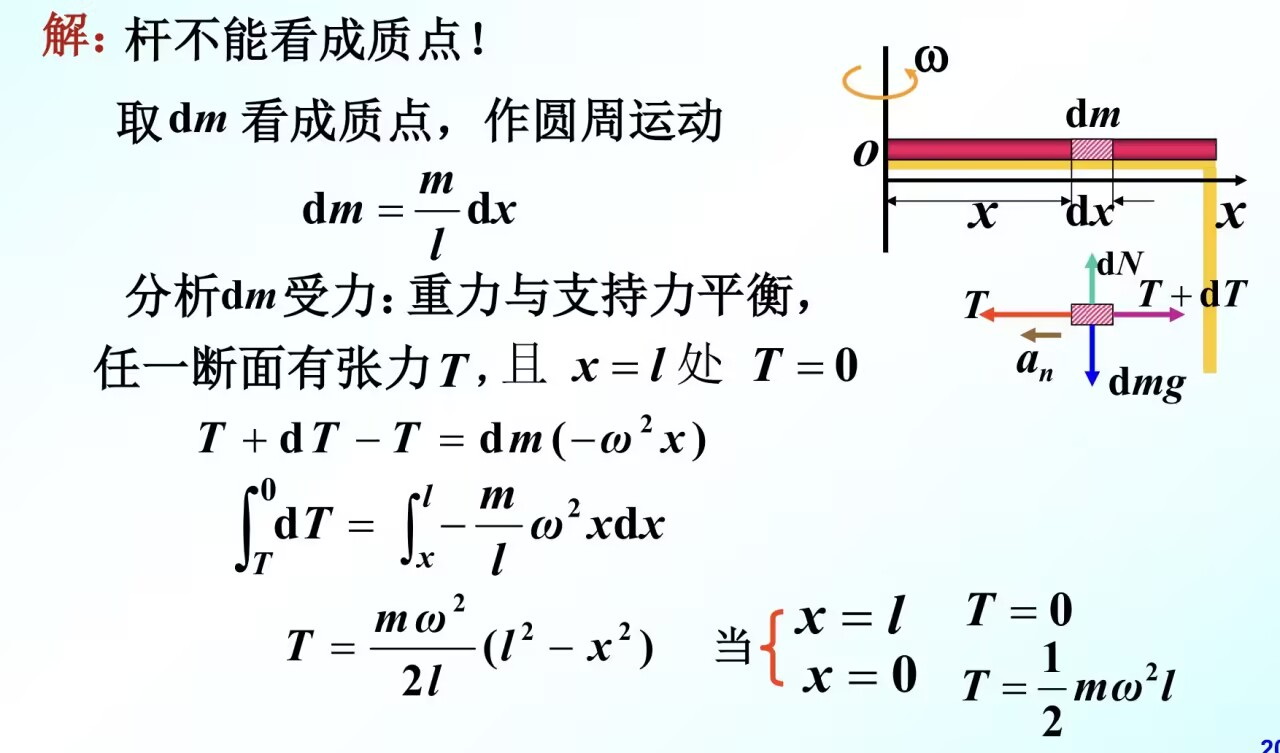
\includegraphics[width=0.8\textwidth]{eg2.jpg}
\end{figure}

例3
\begin{figure}[h]
    \centering
    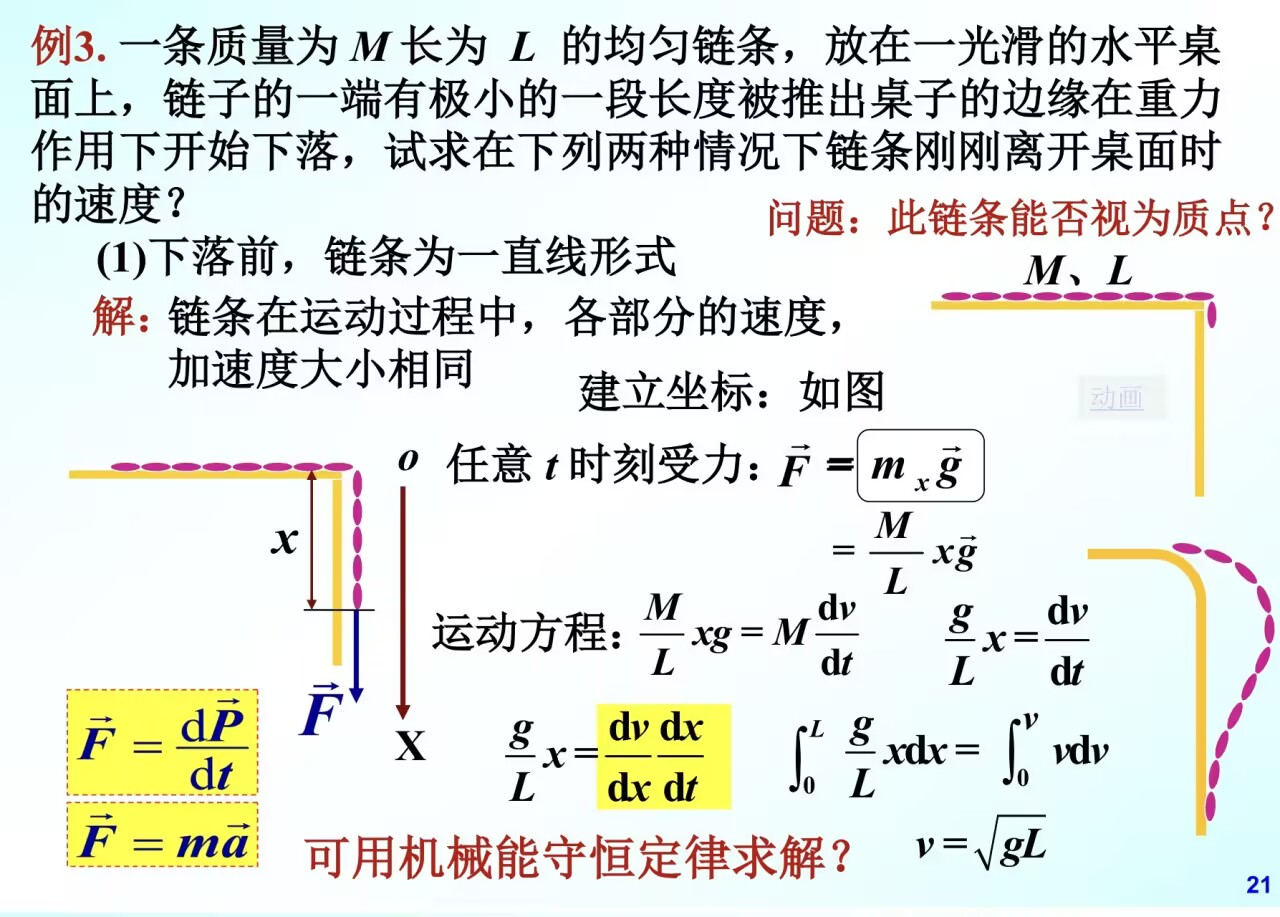
\includegraphics[width=0.8\textwidth]{eg3-1.jpg}
    \end{figure}
\newpage
例3情形2:
\begin{figure}[h]
    \centering
    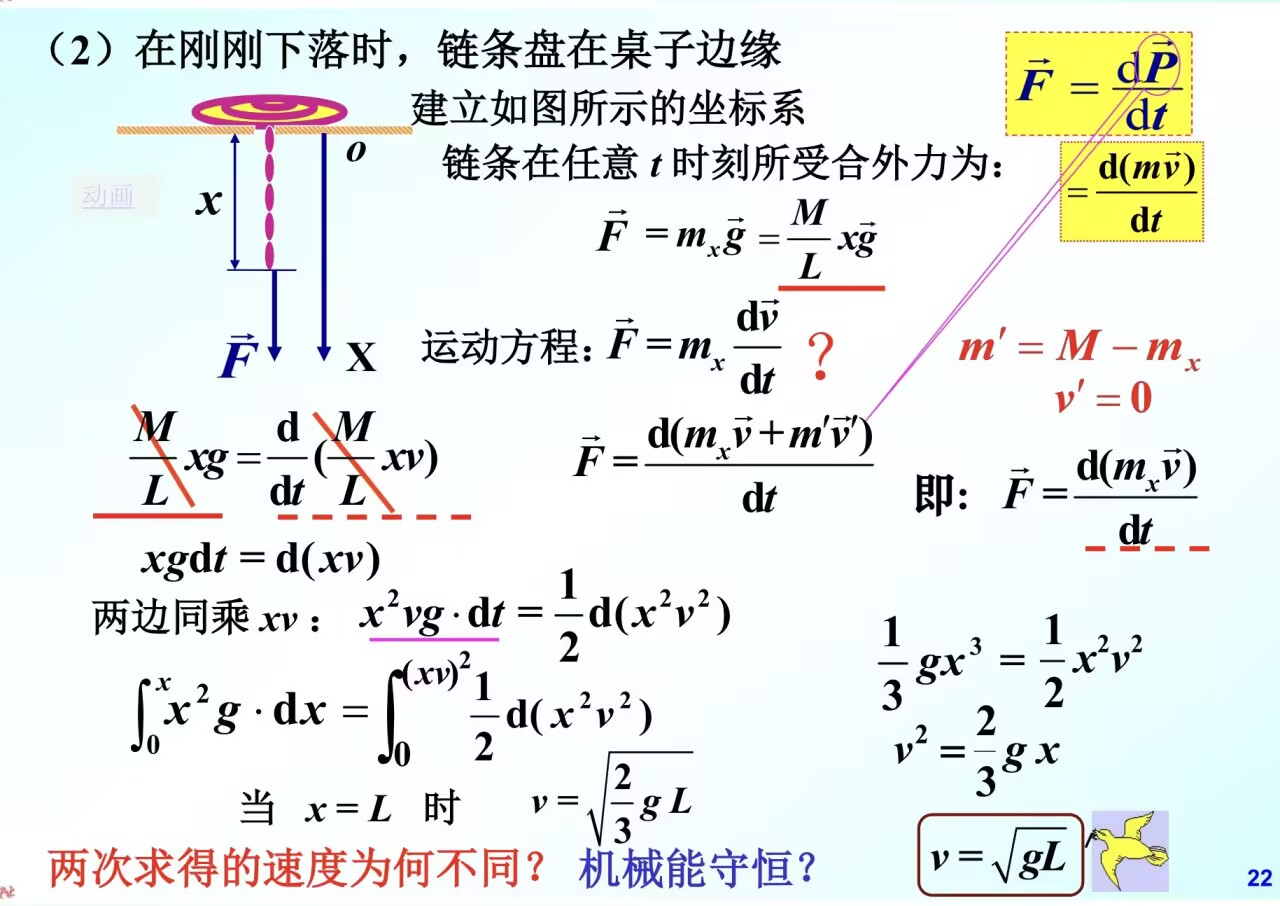
\includegraphics[width=0.8\textwidth]{eg3-2.jpg}
    \end{figure}

例4:
\begin{figure}[h]
    \centering
    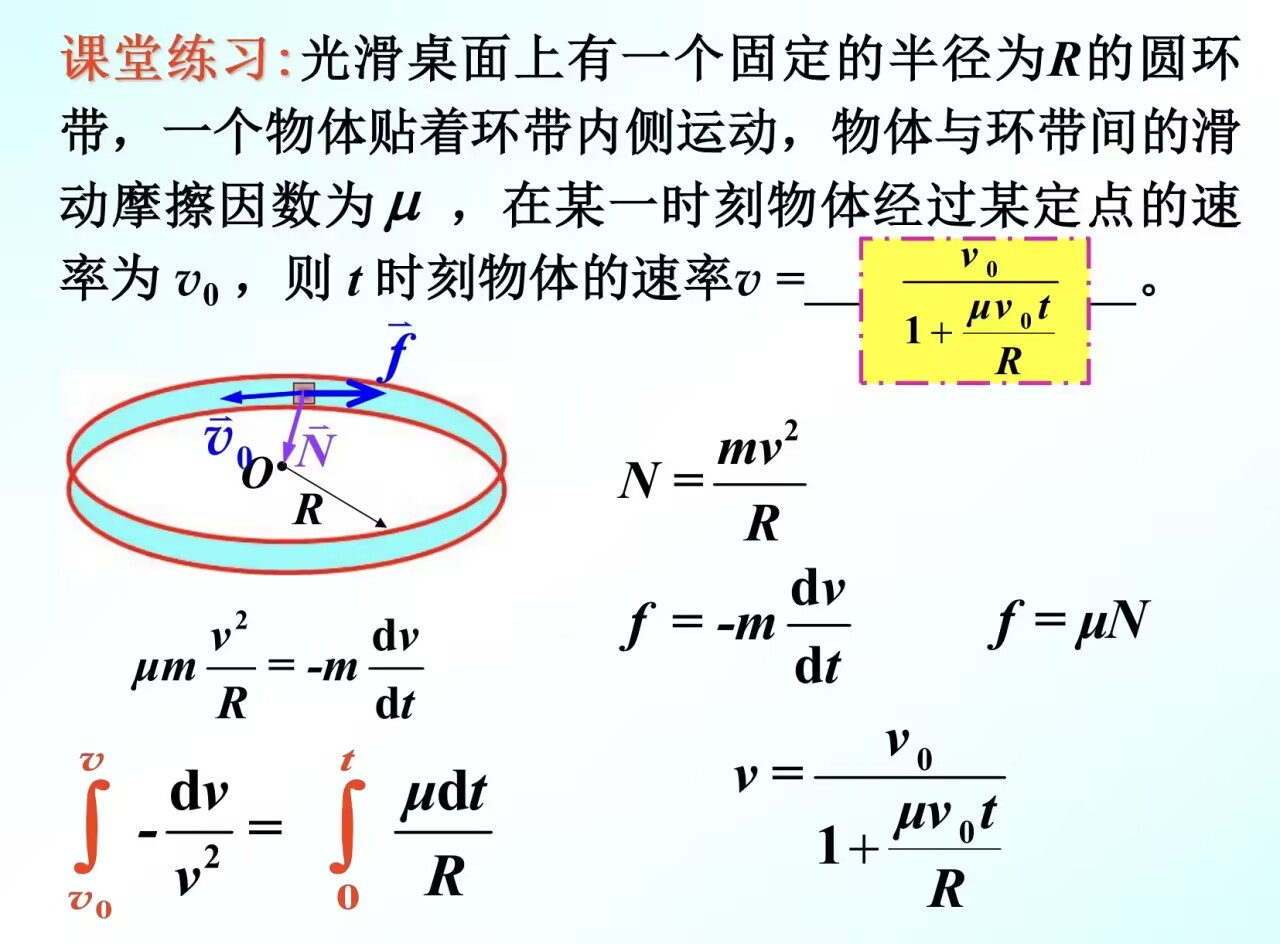
\includegraphics[width=0.8\textwidth]{eg4.jpg}
    \end{figure}
\newpage
例5:
一铅直悬挂的匀质柔软细绳长为$L$,下端刚好触及水平桌面,现松开绳的上端,让绳落至桌面上。
试证明:任意时刻作用于桌面的压力$N$,等于已落到桌面上的绳重$G$的三倍?

\noindent 解:
$dy$下落:
\[Fdt=\Delta P=vdm=\frac{dy}{dt}\frac{m}{L}dy
\Rightarrow
F=\frac{m}{L}(\frac{dy}{dt})^2=\frac{m}{L}v^2
\]
又$v^2=2gy$,有:
\[F=2\frac{y}{L}mg\]
其中$F$为桌面对绳的力.由牛顿第三定律,绳对桌面的力也为$F$.
又$G=\frac{y}{L}mg$,则压力$N=G+F=3G$.\\
不要忘了加G.

例6:
水平桌面上盘放着一根不能拉伸的均匀柔软的长绳,单位长度质量为$\lambda$,
用手将绳的一段以恒定速率$v_0$竖直上提.求提起的绳长为$L$时,手的提力的大小$F$.
\\\textbf{变质量问题,用密尔歇斯基方程!}

\noindent 解:
\[
F-mg=m\frac{dv}{dt}-u\frac{dm}{dt}=v_0\frac{dm}{dt}\]
\[m=\lambda L\Rightarrow \frac{dm}{dt}=\lambda \frac{dy}{dt}=\lambda v_0\]
\[\Rightarrow F=mg+v_0^2 \lambda=\lambda Lg+\lambda v_0^2\]

\noindent 另解:设$t$时刻提起的绳长为$y$,$t+dt$时刻提起的绳长为$y+dy$\\
对于长为$y+dy$的绳(看作质点系):
\[(F-mg)dt=(y+dy)\lambda v_0-y\lambda v_0=\lambda v_0dy\]
\[\Rightarrow F=mg+\lambda v_0\frac{dy}{dt}=\lambda Lg+\lambda v_0^2\]

例7:
长为$l$的铁链平放在桌上,质量线密度为$\rho$,
用手提起链的一段使之以匀速$v_0$铅直上升,
求:从一段离地到全链离地,手的拉力的冲量?

\noindent 解一:
同例6可得\[F=\rho yg+\rho v_0^2\]
\[\Rightarrow I_F=\int_0^{\frac{l}{v_0}}Fdt
=\int_0^{\frac{l}{v_0}}(\rho v_0tg+\rho v_0^2)dt
=\frac{\rho gl^2}{2v_0}+\rho v_0l\]
\noindent 解二:动量定理
\[\int_0^t(F-\rho gy)dt=\rho lv_0
\Rightarrow I_F=\int_0^tFdt=\frac{\rho gl^2}{2v_0}+\rho v_0l\]

例8:
用角动量守恒定律推导开普勒第二定律.
\[dS=\frac{1}{2}\lvert \vec{r}\times d\vec{r}\rvert
\Rightarrow \frac{dS}{dt}=\frac{1}{2}\lvert \vec{r}\times \frac{d\vec{r}}{dt}\rvert
=\frac{1}{2}\lvert \vec{r}\times \vec{v}\rvert
=\frac{\vec{L}}{2m}
\]\\
$\vec{L}$为常矢量,则$\frac{dS}{dt}$为常量,且行星的运动为平面运动($\vec{L}$方向不改变)

\end{document}